\documentclass[10pt]{beamer}

\usetheme{m}

\usepackage{subcaption}
\usepackage{booktabs}
\usepackage[scale=2]{ccicons}

\usepackage{pgfplots}
\usepgfplotslibrary{dateplot}

\setlength\parindent{0pt}
\graphicspath{{./figures/}}

\title{Vibrating {\rmfamily\textsc{MEMS}} Gyroscopes}
\date{\today}
\author{Salah Missri}
\institute{EPFL}

\begin{document}

\maketitle

\begin{frame}
  \frametitle{Table of Contents}
  \setbeamertemplate{section in toc}[sections numbered]
  \tableofcontents[hideallsubsections]
\end{frame}

\section{Working principle}

\begin{frame}
\frametitle{Vibratory gyroscope: the Coriolis effect}
\begin{columns}
    \begin{column}{.48\textwidth}
        \begin{figure}
            \centering
            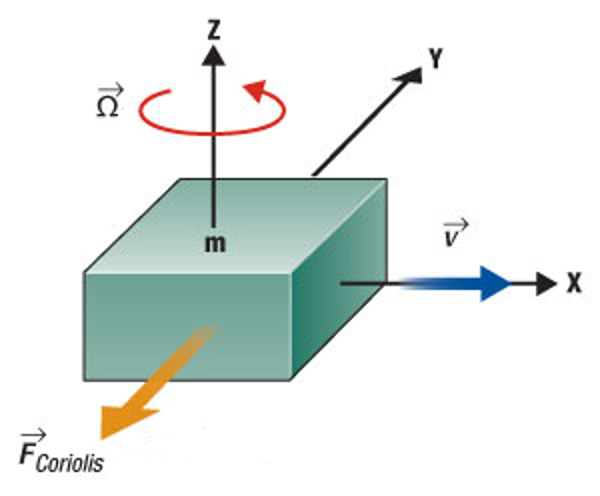
\includegraphics[width=1.\linewidth]{coriolis1.png}
            \caption{Coriolis effect on a mass\cite{MEMSblog}}
        \end{figure}
    \end{column}
    \hfill
    \begin{column}{.60\textwidth}
        \begin{itemize}
            \item Coriolis force is proportional to the angular rate
            \begin{equation*}
                \mathbf{F_{Coriolis} = - 2 m \mathbf{\omega} \times \mathbf{v}}
            \end{equation*}
            \item We can determine $F_{Coriolis}$ by measuring deflection (usually a capacitance measurement)
            \begin{equation*}
                \mathbf{\omega} \propto \mathbf{F_{Coriolis}} \to \mathbf{F} \propto \mathbf{x} \propto \mathbf{C}
            \end{equation*}
            \item But this will also measure linear acceleration
            \begin{equation*}
                \mathbf{F \neq F_{Coriolis}}
            \end{equation*}
        \end{itemize}
    \end{column}
\end{columns}
\end{frame}

\begin{frame}
\frametitle{Tuning fork gyroscope (1/2)}
\begin{columns}
    \begin{column}{.48\textwidth}
        \begin{figure}
        \centering
            \begin{subfigure}[t]{0.9\textwidth}
                \centering
                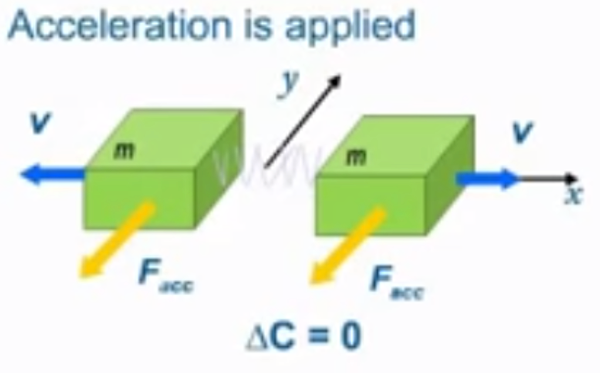
\includegraphics[width=\linewidth]{GyroAcc.png}
            \end{subfigure}
            ~
            \begin{subfigure}[t]{0.9\textwidth}
                \centering
                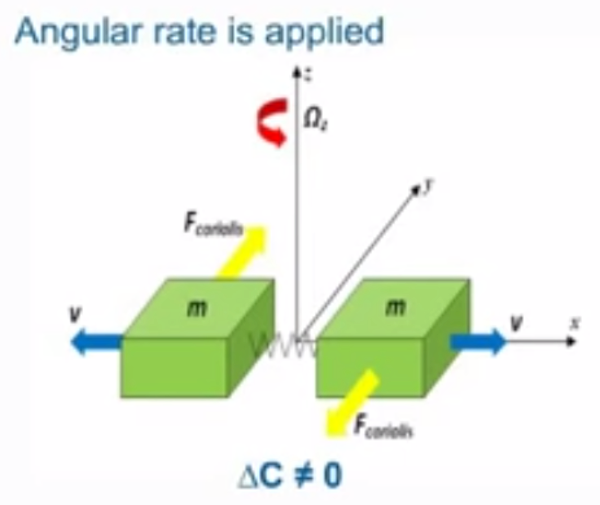
\includegraphics[width=\linewidth]{GyroAngRate.png}
            \end{subfigure}
        \caption{Tuning fork configuration}
        \end{figure}
    \end{column}
    \hfill
    \begin{column}{.60\textwidth}
        \begin{itemize}
            \item Using two coupled masses vibrating in antiphase (tuning fork configuration)
            \begin{equation*}
                \mathbf{F_{Coriolis, 1}} = - 2 m \mathbf{\omega} \times \mathbf{v} = \mathbf{F_{Coriolis, 2}}
            \end{equation*}
            \item Measure the difference between the two masses
            \begin{equation*}
                \mathbf{\omega} \propto \mathbf{F_{Coriolis}} \propto \Delta \mathbf{F} \propto \Delta \mathbf{x} \propto \Delta \mathbf{C}
            \end{equation*}
            \item Isolates Coriolis force measurement from linear acceleration
        \end{itemize}
    \end{column}
\end{columns}
\end{frame}

\begin{frame}
\frametitle{Tuning fork gyroscope (2/2)}
\begin{columns}
    \begin{column}{.45\textwidth}
        \begin{figure}
            \centering
            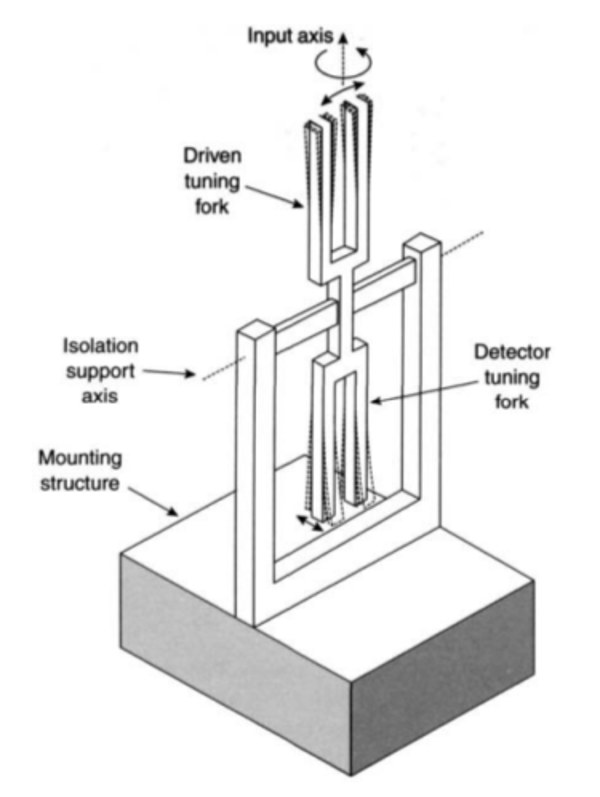
\includegraphics[width=0.9\linewidth]{quartz_rate_gyro.png}
            \caption{Quartz rate sensor\cite{Titterton}}
        \end{figure}
    \end{column}
    \hfill
    \begin{column}{.70\textwidth}
        \begin{figure}
            \centering
            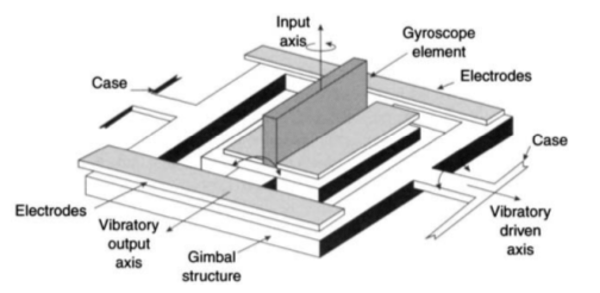
\includegraphics[width=1.0\linewidth]{silicon_gyro.png}
            \caption{1D MEMS gyroscope\cite{Titterton}}
        \end{figure}
    \end{column}
\end{columns}
\end{frame}

\section{Limitations}

\begin{frame}
\frametitle{Limitations}
    For the single 1D sensors
    \begin{itemize}
        \item Sensitive to change in ambient temperature
    \end{itemize}

    For 3D sensing using 1D sensors
    \begin{itemize}
        \item Alignement issues (getting the sensors at exactly $90^{\circ}$)
        \item Getting the same vibration frequency for all three masses
        \item Cross-talk particularly if all three sensors are on the same substrate (also present if other types of vibrating sensors are used)
    \end{itemize}
\end{frame}

\begin{frame}
\frametitle{Multi-axis gyroscope sensors}
\begin{columns}
    \begin{column}{.60\textwidth}
        \begin{figure}
            \centering
            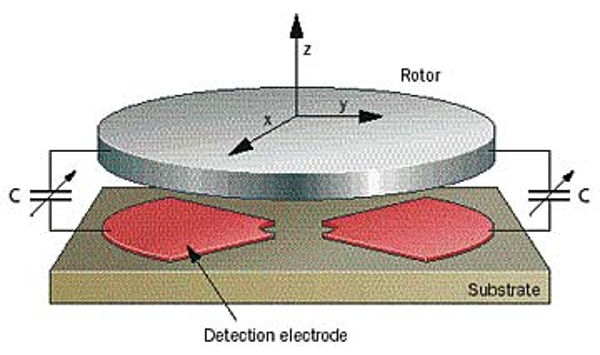
\includegraphics[width=1.0\linewidth]{vibrating_disk.png}
            \caption{Vibrating disk gyroscope (2D)}
        \end{figure}
    \end{column}
    \hfill
    \begin{column}{.50\textwidth}
        \begin{figure}
            \centering
            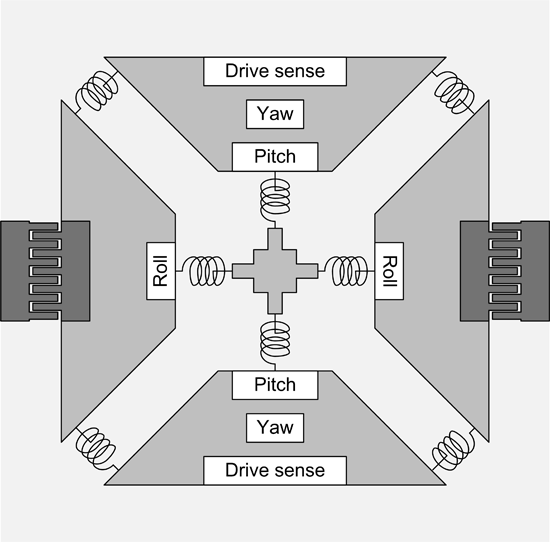
\includegraphics[width=1.0\linewidth]{gyro_mems_3in1.png}
            \caption{3D MEMS gyroscope}
        \end{figure}
    \end{column}
\end{columns}
\end{frame}

\section{Advantages \& drawbacks}

\section{Performances \& applications}

\section{References}

\begin{frame}[allowframebreaks]
\frametitle{References}
    \bibliography{presentation}
    \bibliographystyle{abbrv}
\end{frame}

\plain{Thank you for your attention\\Questions?}


\end{document}
